Die Markov-Eigenschaft erhält ein eigenes Kapitel, da sie wichtig zum Verständnis dieser Arbeit ist und bei der Modellierung eines Reinforcement Learning Problems eine besondere Rolle spielt. Verbinden lässt sich dies sehr gut mit einem Einblick über die grundsätzliche Modellierung von Zuständen bei einem Reinforcement Learning Problem.

\begin{quote}
    The future is independent of the past given the present
  \end{quote}

Dieser Satz erscheint oft in der Literatur, wenn es um die Markov-Eigenschaft geht, so z.B. in den Arbeiten von \cite{Feldman2010}, \cite{kumar2014markov}, \cite{capela2019monogamy} und \cite{SaulMarkov}, oder auch in der Vorlesung der Stanford-Professorin Emma \cite{Brunskill}. Er fasst prägnant zusammen, was die Markov-Eigenschaft aussagt. Im Zusammenhang von MDPs lässt sich dieser Satz so übersetzen, dass ein Folgezustand nicht abhängig von Aktionen bzw. Zuständen in der Vergangenheit ist, sondern ausschließlich von dem aktuellen Zustand und der aktuell gewählten Aktion.
\par 
\cite{Sutton1998} sehen die Markov-Eigenschaft als Einschränkung für die Zustände und nicht für den Entscheidungsprozess als solches. 
Ausschlaggebend ist, dass der Zustand, auf dessen Basis der Agent seine Entscheidung trifft, alle notwendigen Informationen der Vergangenheit beinhaltet, die für die Zukunft relevant sind (S.49).
Die Umwelt ist somit nicht notwendigerweise gezwungen, Markov-konforme Zustände zu liefern. \cite{Brunskill} wählt aufgrund dessen die Bezeichnung \glqq Beobachtung\grqq{} (Observation $O_t$) als Feedback der Umwelt nach einer Aktion. Jene Beobachtungen können anschließend durch eine interne Repräsentation zu Markov-Zuständen verarbeitet werden, die dann dem Entscheidungsfinder zugrunde liegen.
\par
Folgendes Beispiel, basierend auf der Vorlesung von \cite{Brunskill}, liefert einen guten Einblick in die Zustandsmodellierung und der Problematik, die mit der Markov-Eigenschaft einhergeht.
\par 
\begin{figure}[H]
  \centering
  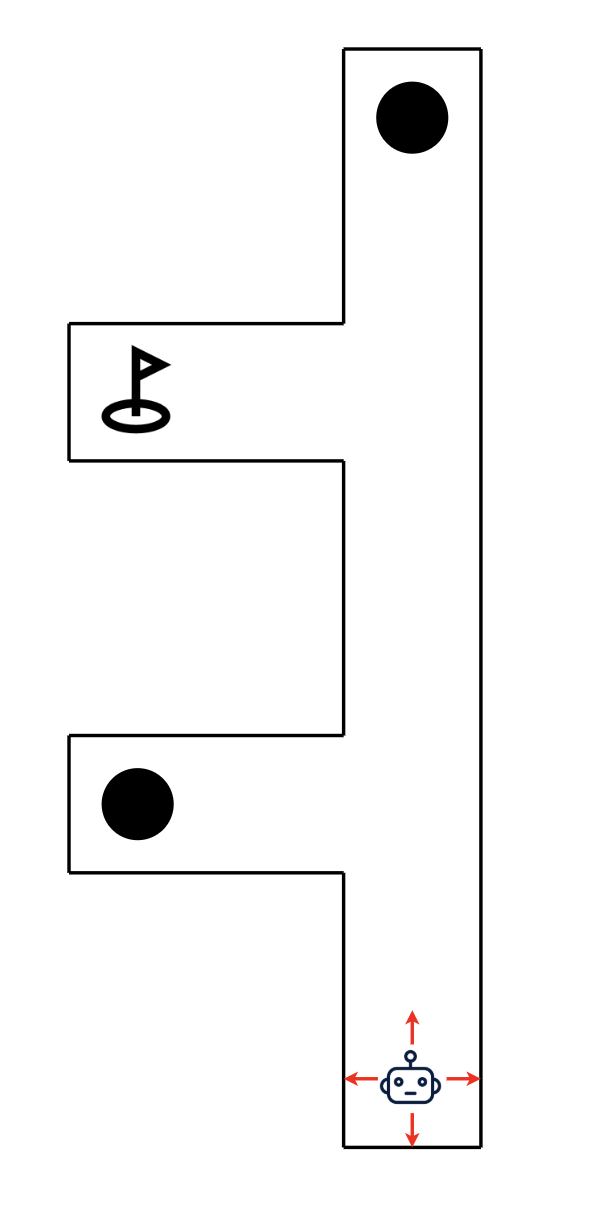
\includegraphics[height=200px]{images/2passagesDefault.png}
  \caption{ Zwei-Wege Beispiel zu der Markov-Eigenschaft}
  \label{fig:2-Wege-1}
\end{figure}

Gegeben ist ein beweglicher Roboter und eine Strecke mit zwei Korridoren. Der Roboter ist mit vier Sensoren ausgestattet, die jeweils eine Himmelsrichtung abdecken. Diese Sensoren sind in der Lage, angrenzende Wände zu erkennen und bilden den Zustand der Umwelt ab. Wahlweise ist der Zustand im Uhrzeiger definiert $\{N, O, S, W\}$, wobei 1 angibt, dass eine Wand erkannt wurde und 0, dass sich keine Wand in der unmittelbaren Nähe befindet. Es ergeben sich folglich 16 unterschiedliche Zustände, die der Agent unterscheiden und auf dessen Basis er Entscheidungen treffen kann (vier Aktionen: Fahrt in jeweils eine Richtung). Der Roboter soll sein Ziel erreichen, markiert mit einer Flagge, ohne dabei in eine der beiden Fallen zu navigieren.
\par
\begin{wrapfigure}{H}{0.5\textwidth}
  \begin{center}
  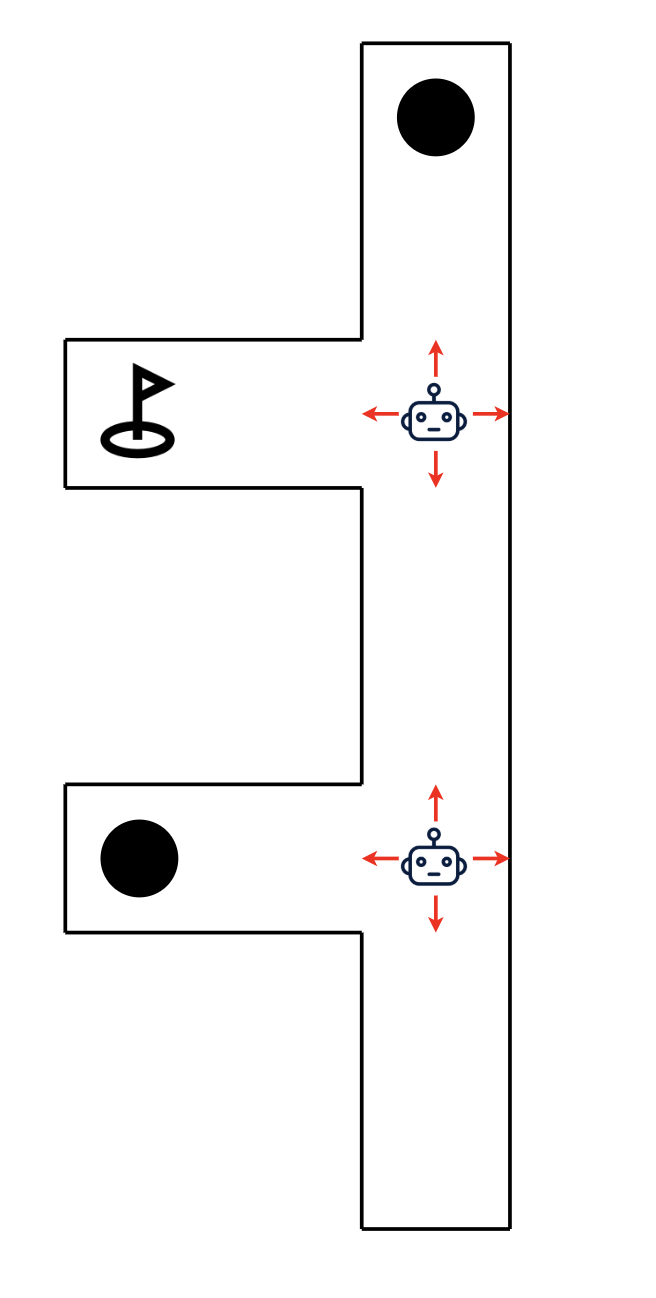
\includegraphics[height=200px]{images/2passagesStart.png}  \end{center}
  \caption{Zwei-Wege Beispiel Forts.}
  \label{fig:2-Wege-2}
\end{wrapfigure}

Eine potenzielle Startposition, wie in Abb. \ref{fig:2-Wege-1} dargestellt, liefert somit den Zustand $\{0, 1, 1, 1\}$. Angenommen der Agent hat gelernt in diesem Zustand Richtung Norden zu fahren, dann ist der Folgezustand ebenfalls $\{0, 1, 1, 1\}$. Schließlich erreicht er den ersten Korridor. Der westliche Sensor liefert folgerichtig 0 und der Zustand ist $\{0, 1, 0, 0\}$. Da der Agent nicht den ersten Korridor folgen darf, sondern dem zweiten, muss der Zustand $\{0, 1, 0, 0\}$ ebenfalls die Aktion \glqq nach Norden fahren\grqq{} auslösen. Das Besondere hier ist jedoch, dass der Zustand bei dem zweiten Korridor identisch mit dem Zustand bei dem ersten Korridor ist und der Agent somit keine Chance hat, zu unterscheiden, vor welchem er sich gerade befindet, siehe Abb. \ref{fig:2-Wege-2}. Er würde ebenfalls, wie schon bei dem ersten Korridor, weiter nach Norden und letztendlich in die Falle fahren.
\par 

Bezogen auf diesen Entscheidungsprozess ist die Modellierung der Zustände über den Sensorinput alleine nicht ausreichend, um die gestellte Aufgabe zu lösen. Die Kombination von Aufgabenstellung und dem Format der Zustände in dieser Form erfüllt insofern nicht die Markov-Eigenschaft, dass auf Basis der erkannten Zustände keine Möglichkeit besteht, die optimalen Entscheidungen zu treffen. 
\par

In der Theorie ist es jedoch möglich diesen Entscheidungsprozess als MDP umzumodellieren.
Dazu kann z.B. die gesamte Historie der Zustände und Aktionen gespeichert werden. Dadurch ist der Roboter in der Lage, zurückzuverfolgen, wo er sich zurzeit befindet. Obowhl dies rein theoretisch möglich ist, sollte diese Herangehensweise vermieden werden. Historien als Zustand für eine Entscheidung zu betrachten bedient zwar die Markov-Eigenschaft, ist allerdings in der Praxis nicht praktikabel, da der Zustandsraum auf diese Weise sehr schnell zu große Ausmaße annimmt.
\par 
Eine weitere Möglichkeit besteht darin, die Sensordaten als Beobachtungen der Umwelt zu betrachten und eine interne Repräsentation von Markov-Zuständen zu pflegen. Dabei bildet der Agent die Umwelt nach jeder erhaltenden Beobachtung suk­zes­si­ve nach, wodurch letztendlich ein Gesamtbild der Umgebung entsteht. Diese Form der Zustandsbildung bedarf jedoch zusätzlicher Algorithmen, die zwischen der Wahrnehmung des Agenten und dem jeweiligen RL-Algorithmus sitzen. 
\par 
Zudem ist das Lernen auf diese Weise auf eine bestimmte Umgebung festgelegt. Wird der Roboter mit einer neuer Welt konfrontiert, z.B. eine Welt mit drei Korridoren, so kann er Gelerntes nicht anwenden, weil seine interne Repräsentation invalide ist.
\par 
Letztendlich muss jedes Szenario zu Beginn genau untersucht werden, um zu beurteilen, ob Reinforcement Learning überhaupt auf dieses Problem anwendbar ist. Dabei spielt vor allem die Markov-Eigenschaft eine wichtige Rolle, die Grundvorraussetzung für alle RL-Algorithmen ist. Für eine Bewertung, ob optimales Verhalten durch gegebene Informationen erreicht werden kann,existieren jedoch keine festen Regeln oder eine Blaupause. Es muss auf Erfahrungswerte oder Untersuchungen zu dem Konvergenzverhalten und den Ergebnissen des gelernten Verhaltens zurückgegriffen werden, wie es auch in den Beispielen dieser Arbeit geschieht in dem Kapitel \ref{sec:praktischerTeil}.
